\documentclass{article}
\usepackage{import}
\usepackage[ruled]{algorithm2e}
\usepackage[shortlabels]{enumitem}
\usepackage{hyperref}
\usepackage{minted}
\usepackage{subcaption}

\hypersetup{
    colorlinks=true,
    linkcolor=blue,
    filecolor=magenta,      
    urlcolor=cyan,
    pdftitle={Overleaf Example},
    pdfpagemode=FullScreen,
    }
\subimport*{}{macro}

\setlength\parindent{0px}

\begin{document}
\setcounter{problem}{0}
\title{Homework \#2}
\author{
    \normalsize{AA 597: Networked Dynamics Systems}\\
    \normalsize{Prof. Mehran Mesbahi}\\
    \normalsize{Due: Jan 26, 2024 11:59pm}\\
    \normalsize{Soowhan Yi}
}
\date{{}}
\maketitle


\begin{problem}
    The complement of graph $G = (V,E)$, denoted by $\bar{G}$, is a graph $(V,\bar{E})$, where $uv \in \bar{E}$ if and only if $uw \notin E$. Show that 
    \begin{align*}
        L(G) + L(\bar{G}) = nI -11^T
    \end{align*}
    
    First, by definition, degree matrix of complement of graph $(n-1)I - D(G)$. Assuming that the graph and the complement do not have self loop, complement graph would have a adjacency matrix($A(\bar{G})$) that would make the adjacecny matrix of the graph (($A(G)$)) would become adjacency matrix of complete graph when ($A(\bar{G})$) is added, since the complement of a graph contains edges that would make the union of those graphs to become complete grapoh. Therefore adding their adjacency matrix would result in $11^T - I$.
    \begin{align*}
        L(G) + L(\bar{G}) &= D(G) - A(G) + D(\bar{G}) - A(\bar{G})\\
        &= D(G) + D(\bar{G}) - (A(G)+ A(\bar{G}))\\
        &= D(G) + (n-1)I - D(G)- (A(G)+ A(\bar{G}))\\
        &= (n-1)I - (11^T - I) = nI -11^T
    \end{align*}

    Conclude that for $2 \leq j \leq n$,
    \begin{align*}
        \lambda_j (\bar{G}) = n - \lambda_{n+2-j}(G)
    \end{align*}
    Lets think about the laplacian of complete graph $K_n$, and its eigenvalues. Since the complete graph can be divided into some graph G and its complement, the laplacian of it would equal to $L(G) + L(\bar{G})$. Therefore 
    \begin{align*}
        L(K_n) v_j = (L(G) + L(\bar{G})) v_j = (nI -11^T) v_j
    \end{align*}
    Since the $K_n$ is connected, the eigenvectors are just multiple of ones ($\alpha 1$) for the very first eigenvalue which is 0. This is also applicable to $G$ and $\bar{G}$.
    \begin{align*}
        (nI -11^T) v_j = (L(G) + L(\bar{G})) v_j = L(G) v_j + L(\bar{G}) v_j = \lambda_j(G) v_j + \lambda_j(\bar{G})v_j 
    \end{align*}
    Due to fact that the eigenvectors are independent of each other and eigenvector for 0 eigenvalue is [1]s, the $v_j$ is orthogonal to $11^T$ for $j \geq 2$. Therfore $(-11^T) v_j = 0$. 
    \begin{align*}
        \therefore n = \lambda_j(G) + \lambda_j(\bar{G})
    \end{align*}
    If we were to sort the laplacian spectrum of $\bar{G}$ in increasing order, then $ \lambda_j(\bar{G}) = n - \lambda_{n + 2 - j}(G)$, assuming that the laplacian spectrum of G is already in increasing order. 
\end{problem}

\begin{problem}
    Show that for any graph $G, \lambda_n(G) \geq d_{max}(G)$

    According to Courant Fischer theorum, $\max {x^T A x}= \lambda_n$, where A is a symmetric matrix with $n \times n$ and $||x|| = 1$. Also using eigenvalue decomposition, we can say that $L(G) = Q \Lambda Q^{-1}$, where $\Lambda = \begin{bmatrix}
        0 = \lambda_1 & 0 & 0 & \cdots & 0\\
        0 & \lambda_2 & 0 & \cdots & 0\\
        0 & 0 & \lambda_3 & \cdots & 0\\
        \vdots & & &\\
        0 &  & & &\lambda_n
    \end{bmatrix}$ and $Q = \begin{bmatrix}
        v_1 & v_2 & \cdots & v_n
    \end{bmatrix}$, where $\lambda_1 \leq \lambda_2 \leq \cdots \leq \lambda_n$.  $v_i$ are eigenvectors corresponding to those eigenvalues. However, $L_G$ is symmetric
    and Q is eigenvectors of $L_G$, and therefore Q has to be a orthogonal matrix and $Q^{-1} = Q^{T}$.
    Now we utilize above properties to solve the problem. 
    \begin{align*}
        L(G) = Q \Lambda Q^{-1} = Q \Lambda Q^{T}\\
        x^T L(G) x = x^T  Q \Lambda Q^{T} x
    \end{align*}
    Let $y = Q^T x$, and simplify
    \begin{align*}
        x^T L(G) x = x^T  Q \Lambda Q^{T} x &= y^T \Lambda y\\
        &=\lambda_1 y_1^2 + \lambda_2 y_2^2 + \lambda_3 y_3^2 \cdots + \lambda_n y_n^2
        \leq \lambda_n y_1^2 + \lambda_n y_2^2 + \lambda_n y_3^2 \cdots + \lambda_n y_n^2 = \lambda_n y^ty\\ 
        &\therefore x^T L(G) x \leq \lambda_n (\because y^Ty = x^TQQ^Tx = x^Tx = 1)
    \end{align*}
    Now, let $x^T = \begin{bmatrix}
        0 &0 &0 &0 &\cdots &1 & 0 & \cdots &0
    \end{bmatrix}$, where only ith vertex has the maximum degree in the graph and only ith component in x is 1, so that we can extract the maximum degree out from degree matrix. 
    \begin{align*}
        x^t L(G)x &= x^T (D(G) - A(G)) x \\
        &= x^T(D(G))x - x^TA(G)x \\
        &= d_{max}(G) - A_{ii}(G)\\
        &= d_{max}(G) \leq \lambda_n (G) (\because A_{ii} = 0)
    \end{align*} 

\end{problem}

\begin{problem}
    Simulate the agreement protocol (3.2) for a graph on five vertices. Compare the rate of convegence of protocol as the number of edges increases. Does the convergence of the protocol alw3ays improve when the graph contains more edges? Provide an analysis to support your observation. 
    \begin{figure*}[!ht]
        \centering
        \begin{subfigure}{0.4\textwidth}
            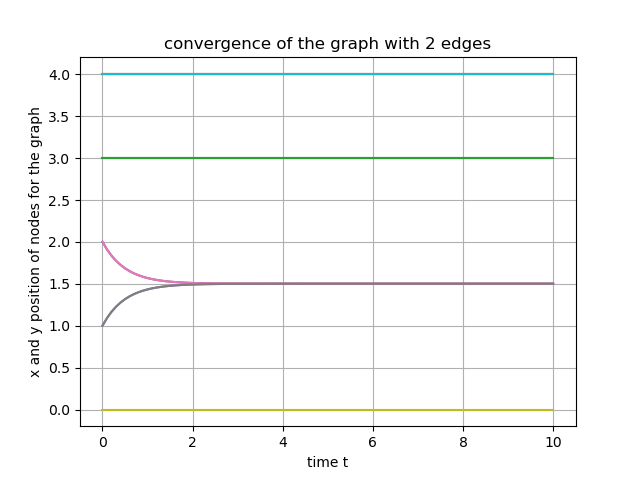
\includegraphics[width=\textwidth]{./img/p3_edge_2_1.png}
            \caption{Graph with 2 edges}
        \end{subfigure}
        \begin{subfigure}{0.4\textwidth}
            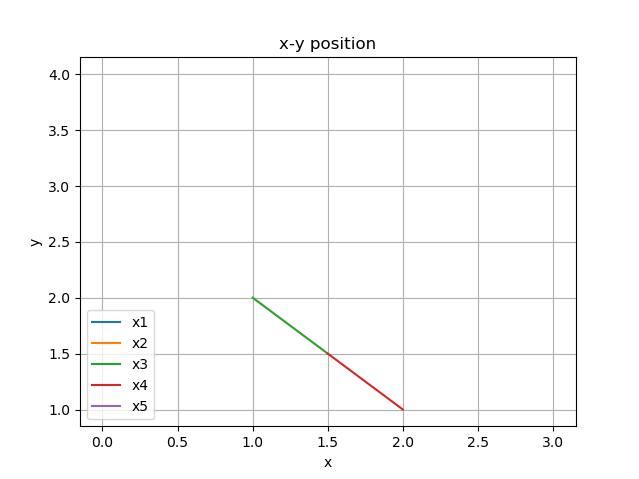
\includegraphics[width=\textwidth]{./img/p3_edge_2_2.png}
            \caption{Graph with 2 edges}
        \end{subfigure}
        \begin{subfigure}{0.4\textwidth}
            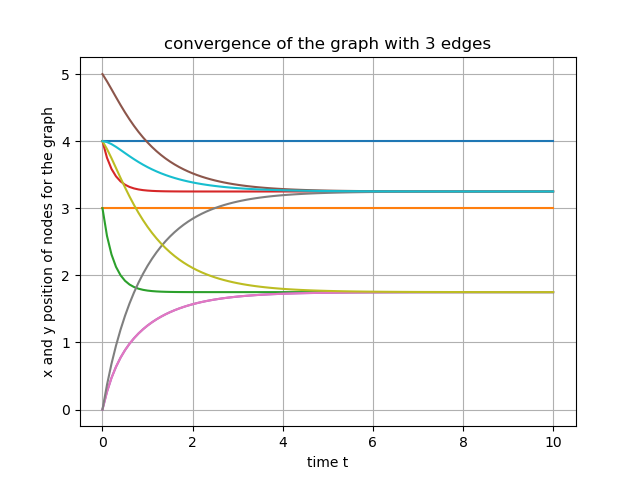
\includegraphics[width=\textwidth]{./img/p3_edge_3_1.png}
            \caption{Graph with 3 edges}
        \end{subfigure}
        \begin{subfigure}{0.4\textwidth}
            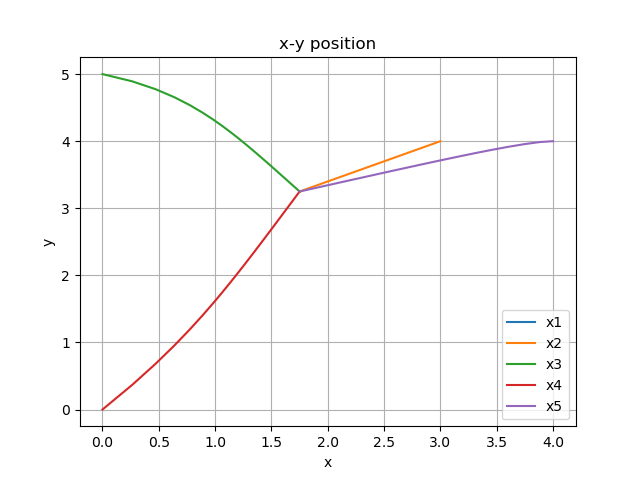
\includegraphics[width=\textwidth]{./img/p3_edge_3_2.png}
            \caption{Graph with 3 edges}
        \end{subfigure}
    \end{figure*}

    \begin{figure*}
        \centering   
        \begin{subfigure}{0.4\textwidth}
            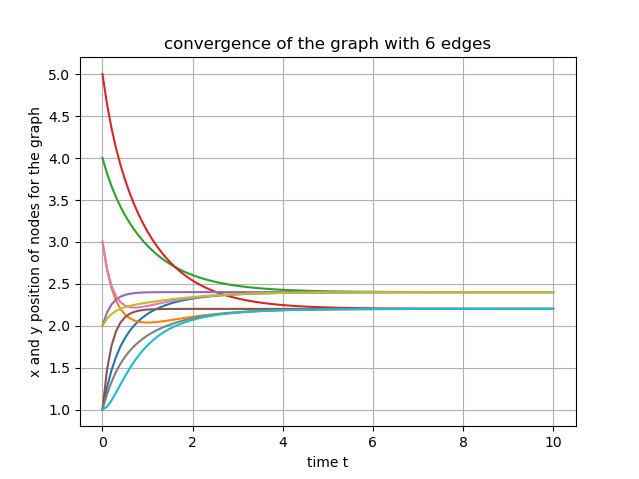
\includegraphics[width=\textwidth]{./img/p3_edge_6_1.png}
            \caption{Graph with 6 edges}
        \end{subfigure}
        \begin{subfigure}{0.4\textwidth}
            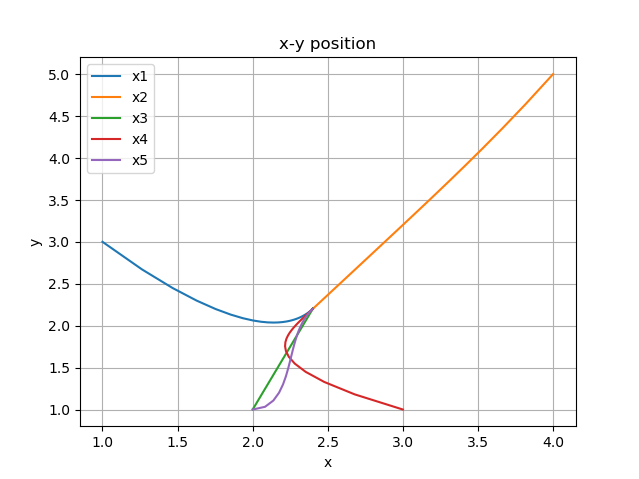
\includegraphics[width=\textwidth]{./img/p3_edge_6_2.png}
            \caption{Graph with 6 edges}
        \end{subfigure}
        \begin{subfigure}{0.4\textwidth}
            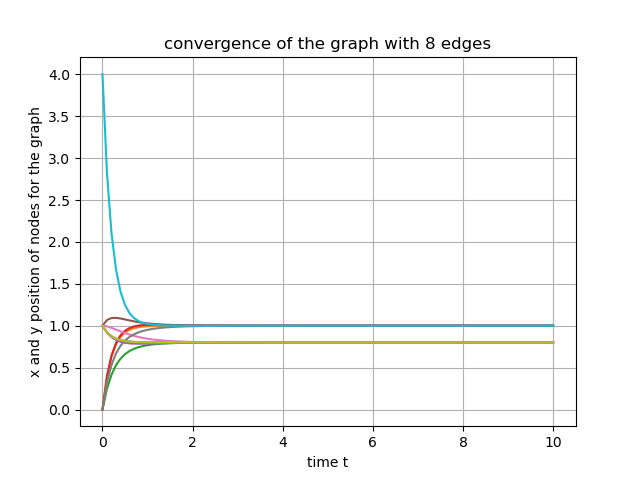
\includegraphics[width=\textwidth]{./img/p3_edge_8_1.png}
            \caption{Graph with 8 edges}
        \end{subfigure}
        \begin{subfigure}{0.4\textwidth}
            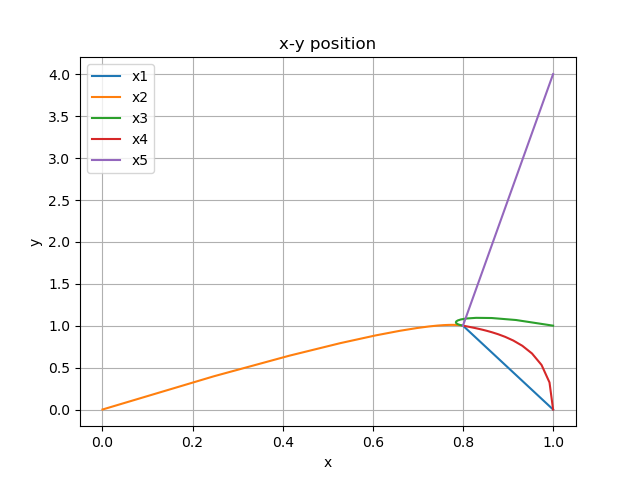
\includegraphics[width=\textwidth]{./img/p3_edge_8_2.png}
            \caption{Graph with 8 edges}
        \end{subfigure}
    \end{figure*}
    \begin{figure*}
        \centering
        \begin{subfigure}{0.4\textwidth}
            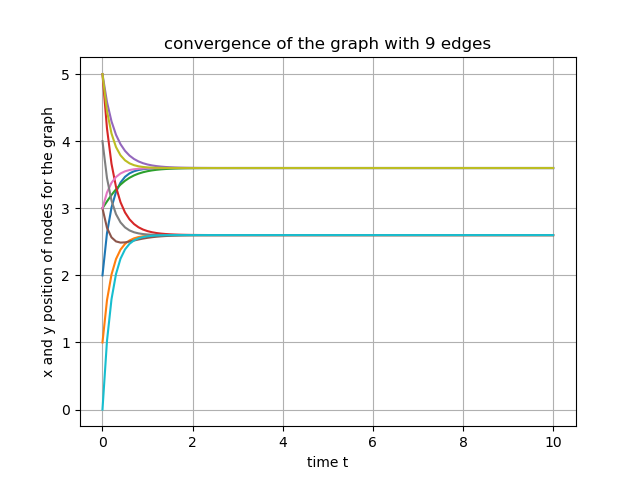
\includegraphics[width=\textwidth]{./img/p3_edge_9_1.png}
            \caption{Graph with 9 edges}
        \end{subfigure}
        \begin{subfigure}{0.4\textwidth}
            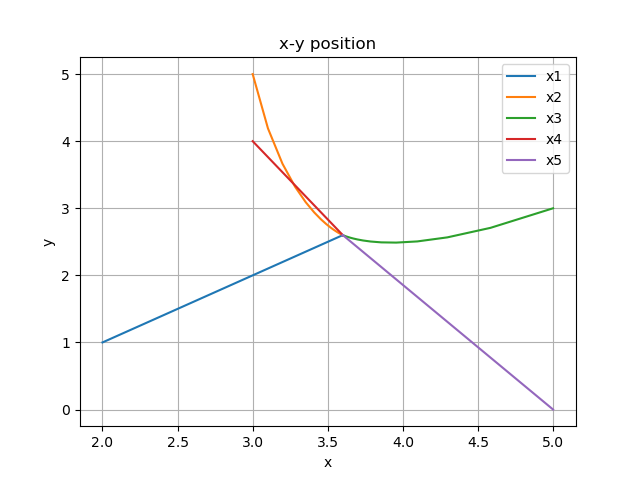
\includegraphics[width=\textwidth]{./img/p3_edge_9_2.png}
            \caption{Graph with 9 edges}
        \end{subfigure}
        \begin{subfigure}{0.4\textwidth}
            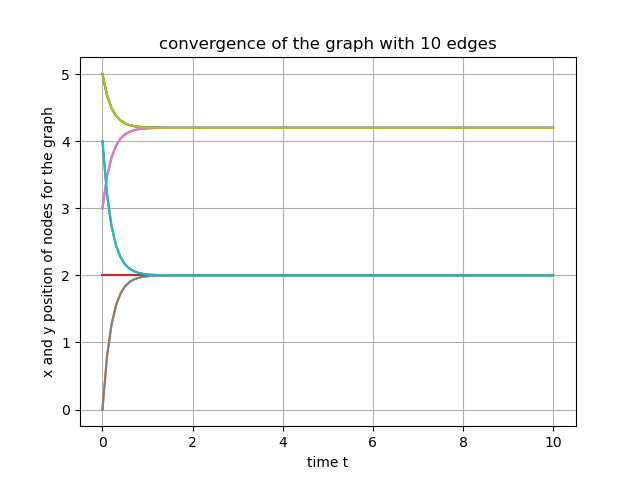
\includegraphics[width=\textwidth]{./img/p3_edge_10_1.png}
            \caption{Graph with 10 edges}
        \end{subfigure}
        \begin{subfigure}{0.4\textwidth}
            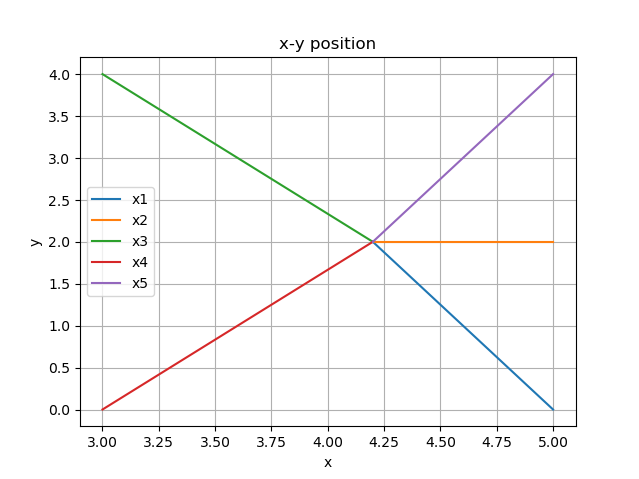
\includegraphics[width=\textwidth]{./img/p3_edge_10_2.png}
            \caption{Graph with 10 edges}
        \end{subfigure}

    \end{figure*}
    \begin{figure*}
        \centering
        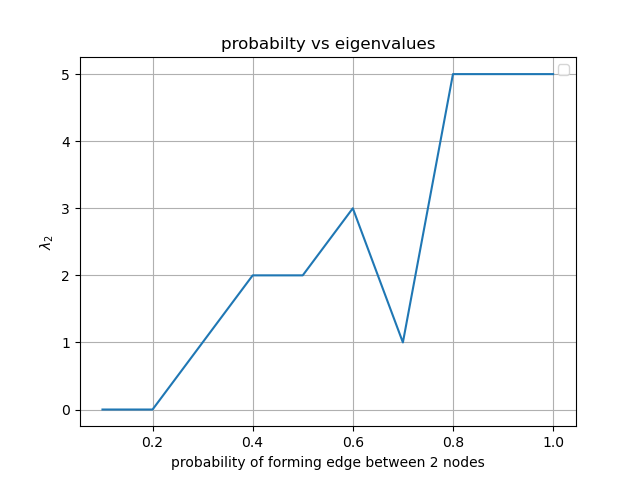
\includegraphics[width=0.5\textwidth]{./img/prob_vs_lambda.png}
        \caption{convergence vs number of nodes}
    \end{figure*}
    \newpage
    As we can see from above figures, we can see that the graphs with more edges are more converging with same number of nodes. Left hand side of above figures show the x and y coordinates seperately in time domain, and the right hand side shows in the x-y plane. As I was not able to create random graph with 5 nodes and spectific number of edges, I created random graph with 5 nodes and used a probability to form an edge between two nodes. As we can see from the last plot, we see that the $\lambda_2$ is increasing as the probability of forming edge between two nodes is increasing. Also from above plots, we see that it converges faster with more edges. Therefore it always improves with more edges. The reason why we have lower eigenvalue at probability equal to 0.7 is that that particular graph did not form enough edges even with 0.7 probabilty. 
\end{problem}
\newpage
\begin{problem}
    \begin{align*}
        \dot{x}_i(t) = \sum_{j \in N(i)} (x_j(t) - x_i(t)), \space i = 1, \cdots , n
    \end{align*}
    How would one modify the agreement protocol (3.1) so that the agents converge to an equilibrium $\bar{x}$, where $\bar{x} = \alpha 1 + d$ for some given $d \in R^n$ and $\alpha \in R$?
    \begin{align*}
        \dot{x}_i(t) = \sum_{j \in N(i)} (x_j(t) - x_i(t)) - k_i(x_i(t) - \bar{x}(t))
    \end{align*}
    I would introduce control term k like above. This way the $\dot{x}_i(t)$ would become zero when$ x_i(t) = \bar{x}(t)$, therefore reaching the equilibrium $\bar{x} = \alpha 1 + d$.
    Control term k can be adjusted for control objectives, but, by introducing $x_i(t) - \bar{x}(t)$, the agents are able to converge to  $\bar{x} = \alpha 1 + d$.
\end{problem}
\begin{problem}
    The second-order dynamics of a unit paticle i in one dimension is 
    \begin{align*}
        \frac{d}{dt} 
        \begin{bmatrix*}
            p_i(t)\\
            v_i(t)  
        \end{bmatrix*}
        = \begin{bmatrix*}
            0 & 1\\
            0 & 0 
        \end{bmatrix*}
        \begin{bmatrix*}
            p_i(t)\\
            v_i(t)  
        \end{bmatrix*}
        + 
        \begin{bmatrix*}
            0\\
            1
        \end{bmatrix*} u_i(t)
    \end{align*}
    where $p_i$ and $v_i$ are, respectively the position and the velocity of the particle with repect to an ineartial frame, and $v_i$ is the force and/or control term acting on the particle. Use a setup, inspired by the agreement protocol, to propose a control law $-u_i(t)$ for each vertex such that: (1) the control input for particle i relies only on the relative posistion and velocity information with respect to its neighbors; (2) the control input to each particle results in an asymptotically cohesive behavior for the particle group, that is, the position of the particle remain close to each other; and (3) the control input to each particle results in having a particle group that evolves twith the same velocity. Simulate you r proposed control law.

\end{problem}

\begin{problem}
    Write a code that implements the consensus protocol  $\dot{x}=-L(G) x$, where L(G) is the Laplacian matrix of the graph,  from arbitrary (random) initial conditions. Use networkX or something similar to run the consensus dynamics on a cycle, path, star, and complete graphs. Find the second smallest eigenvalues of these graphs and see if the convergence properties of consensus  can be matched to these second smallest eigenvalues. Then explore the convergence as a function the number  nodes in these graphs- again using networkX or something similar, choose graphs of sizes 5, 10, 20, and 50 for your computational experiments.
    \begin{minted}{python3}
    def get_xdot(positions, t, L_G):
        num = int(len(positions)/2)
        positions = positions.reshape(num, 2)
        return (-np.matmul(L_G,positions)).reshape(num*2)
        
    def main():
        num = 50
        graphs = [nx.cycle_graph(num),nx.path_graph(num), nx.star_graph(num), nx.complete_graph(num)]
        graph = nx.complete_graph(num)
        graph, positions = random_graphs_init(graph)
        t = np.linspace(0,10,101)
        L_G = nx.laplacian_matrix(graph).toarray()
        trajectory = sp.integrate.odeint(get_xdot, np.reshape(positions, 2*len(graph)), t, args=(L_G, ))
    \end{minted}
    From below graphs, we can see that positions of nodes converge to 2 different numbers because I am using x and y coordinates to show this convergence. Plot below would be more helpful for visualization. But we can see that the position is converging to the agreement. The first 4 plots show the convergence of each x and y position, and the last 4 plots show that the convergence in 2 d plane. 
    
    Also we can see from figure 2,  that $\lambda_2$ is growing for all the graphs when number of nodes are increased. All the plots are included in next page. 
    \begin{figure*}[!ht]
        \centering
        \begin{subfigure}{0.4\textwidth}
            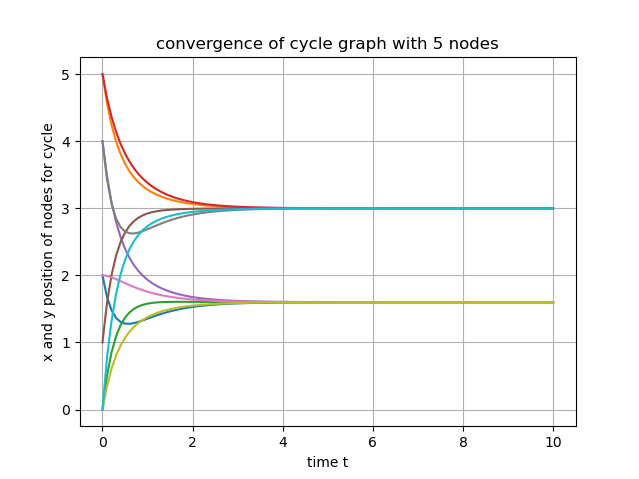
\includegraphics[width=\textwidth]{./img/p1convergence_cycle_graph_5.png}
            \caption{cycle graph}
        \end{subfigure}
        \begin{subfigure}{0.4\textwidth}
            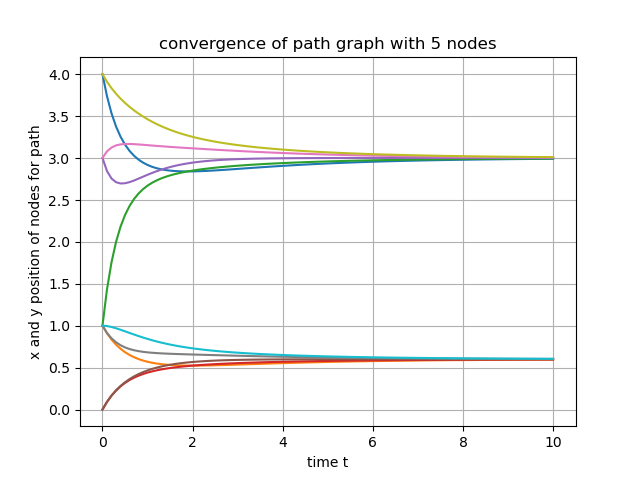
\includegraphics[width=\textwidth]{./img/p1convergence_path_graph_5.png}
            \caption{path graph}
        \end{subfigure}
        \begin{subfigure}{0.4\textwidth}
            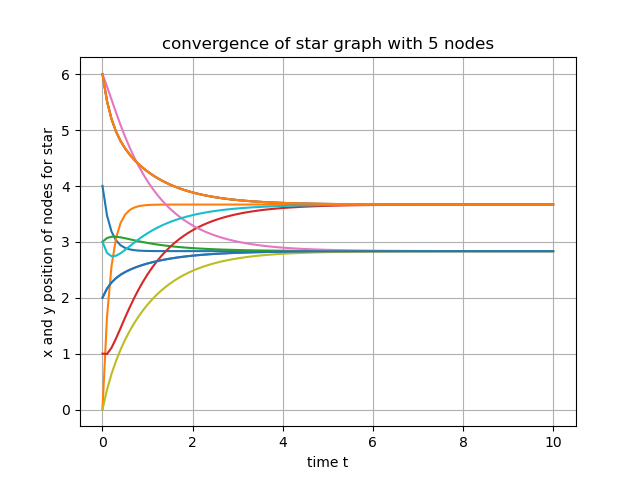
\includegraphics[width=\textwidth]{./img/p1convergence_star_graph_5.png}
            \caption{star graph}
        \end{subfigure}
        \begin{subfigure}{0.4\textwidth}
            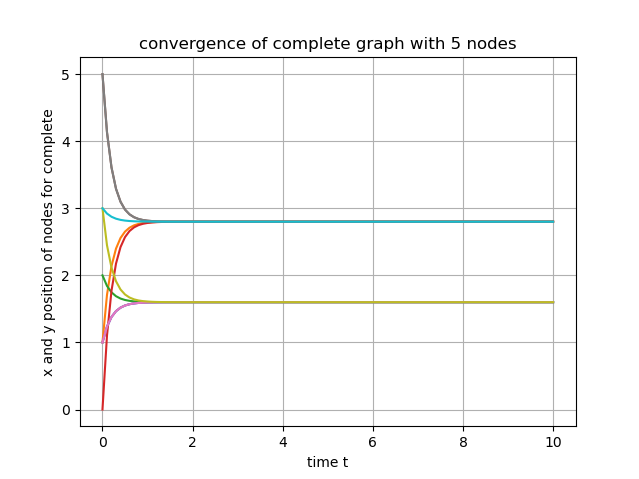
\includegraphics[width=\textwidth]{./img/p1convergence_complete_graph_5.png}
            \caption{complete graph}
        \end{subfigure}

        \begin{subfigure}{0.4\textwidth}
            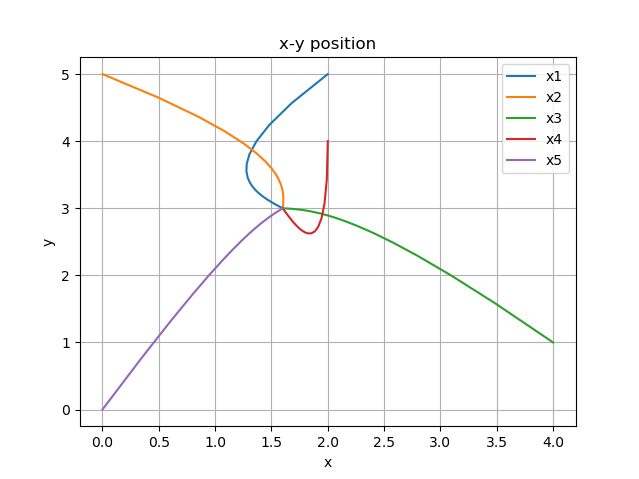
\includegraphics[width=\textwidth]{./img/p1xyposition_cycle_graph_5.png}
            \caption{cycle graph}
        \end{subfigure}
        \begin{subfigure}{0.4\textwidth}
            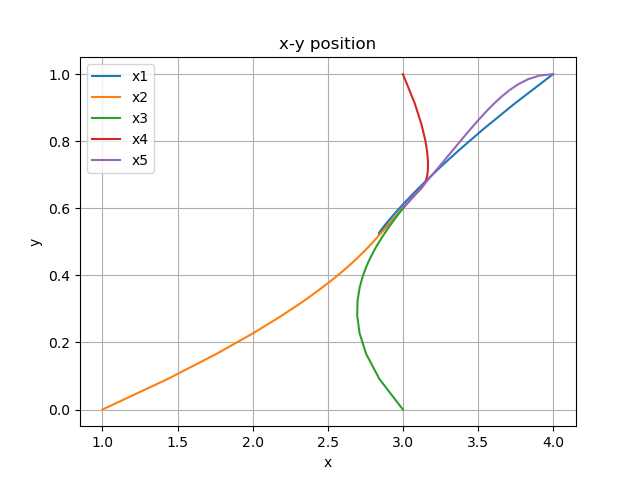
\includegraphics[width=\textwidth]{./img/p1xyposition_path_graph_5.png}
            \caption{path graph}
        \end{subfigure}
        \begin{subfigure}{0.4\textwidth}
            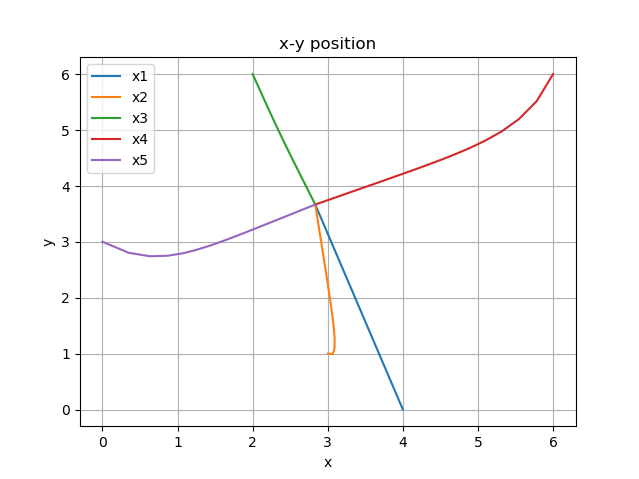
\includegraphics[width=\textwidth]{./img/p1xyposition_star_graph_5.png}
            \caption{star graph}
        \end{subfigure}
        \begin{subfigure}{0.4\textwidth}
            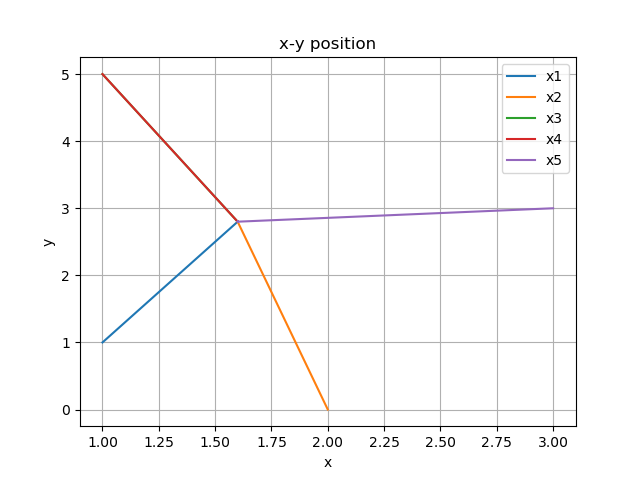
\includegraphics[width=\textwidth]{./img/p1xyposition_complete_graph_5.png}
            \caption{complete graph}
        \end{subfigure}
    \end{figure*}
    \begin{figure*}
        \centering
        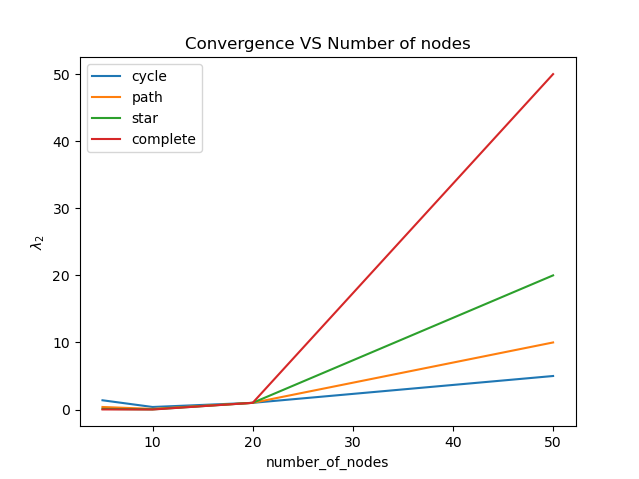
\includegraphics[width=\textwidth]{./img/p1convergence_num_node.png}
        \caption{convergence vs number of nodes}
    \end{figure*}
\end{problem}

\end{document}